\chapter{Автоматизированное создание карт помещений} \label{ch:6}

\section{Введение}\label{sect:6_1}
Поскольку помещения могут быть разных размеров и форм, требуется иметь механизм генерирования карты необходимых элементов, таких как столы и ячейки с продуктами, для любого помещения. Подразумеваются стандартизированные размеры мебели. Таким образом роботу не понадобится дополнительных датчиков, для построения карты помещения в режиме реального времени, что уменьшает стоимость создания и внедрения технологии.

\section{Язык макросов XACRO}\label{sect:6_2}
\textit{ROS} предоставляет удобный механизм создания моделей роботов и карт местности с помощью XML файлов. Но такой подход тяжело параметризируется, поэтому для того, чтобы предоставить пользователям большую гибкость был разработан XML подобный язык макросов XACRO. Он позволяет добавлять в модели роботов параметры, устанавливаемые извне, на выходе обработчика макросов получается обычный файл модели URDF. Кроме того, используя макросы, возможно рекурсивно создавать неограниченное количество объектов. Эта возможность и была использована для создания стандартизированных карт помещений. 

На данный момент создано лишь два высокоуровневых макроса:
\begin{itemize}
	\item add\_table - макрос добавляющий в помещение стол. Принимает в качестве параметров положение, масштабирующий коэффициент и координатную систему родителя.
	\item cells\_group\_macro - макрос добавляющий набор ячеек в помещение. Принимает в качестве параметров положение, масштабирующий коэффициент, систему координат родителя, а также длину, ширину и высоты, выраженные к количестве ячеек.
\end{itemize}

Если добавление стола реализуется довольно просто, то создание ячеек намного более трудоемко. Поскольку каждая группа ячеек состоит из нижнего слоя подставок, поднимающих контейнеры на минимальный доступный манипулятору уровень, а также самих ячеек связанных между собой.

К примеру приведенный в \ref{list:xacro_xml} листинг генерирует карту, изображенную на рисунках \ref{fig:6_2_1} и \ref{fig:6_2_2}.
\begin{figure}[h!]
	\centering
	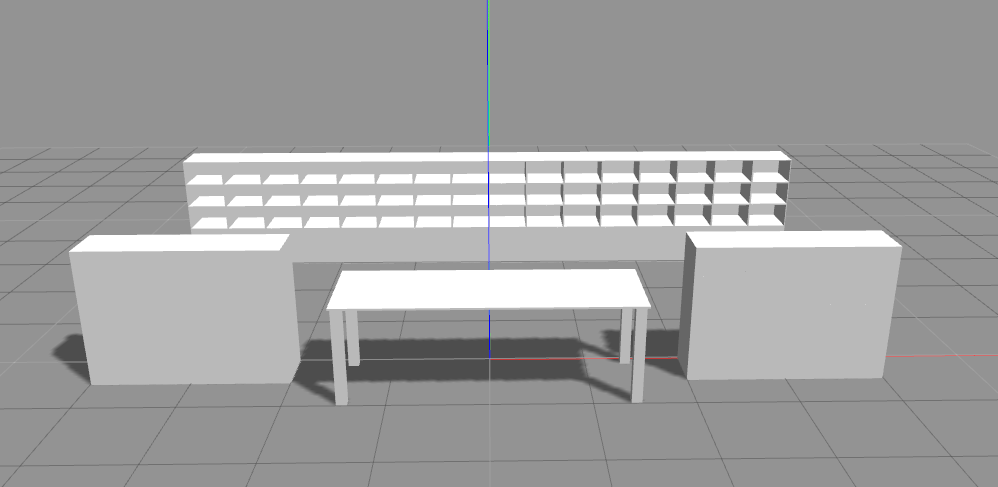
\includegraphics[scale=0.5]{Maps/map_front}
	\caption{Сгенерированная карта. Вид спереди.}
	\label{fig:6_2_1}
\end{figure}
\begin{figure}[h!]
	\centering
	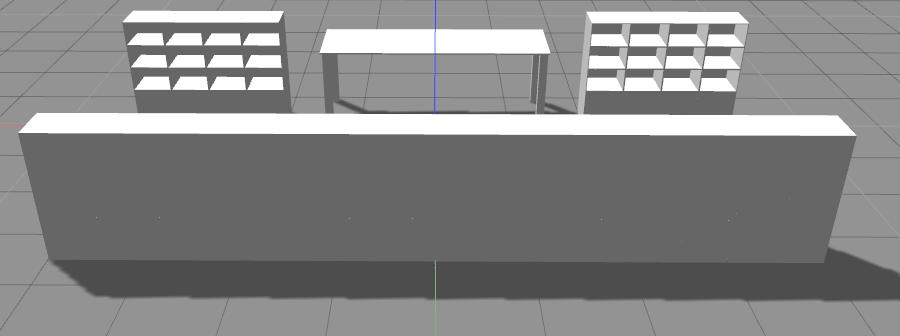
\includegraphics[scale=0.5]{Maps/map_back}
	\caption{Сгенерированная карта. Вид сзади.}
	\label{fig:6_2_2}
\end{figure}
При этом отформатированный(пробелы, здесь есть пробелы между строчками) XACRO код длиной в 44 строки разворачивается в неформатированный(пробелы, здесь нет пробелов между строчками) URDF код, имеющий 2465 строк. Довольно эффективное упрощение, не правда ли?